\section{Beispielrechnung}
\rhead{Beispielrechnung}

\subsection{Einführung}
In diesem Abschnitt wird die Theorie vom Abschnitt \ref{sta} in einem Praxisbeispiel angewendet. 
Wir haben die Deklination, Rektaszension, Höhe der beiden Planeten Deneb und Arktur und die Sternzeit von Greenwich als Ausgangslage.
Die Deklinationen und Rektaszensionen sind von einem vergangenen Datum und die Höhe der Gestirne und die Sternzeit wurden digital in einer Stadt in Japan mit den Koordinaten 35.716672 N, 140.233336 E bestimmt.
Wir werden nachrechnen, dass wir mit unserer Methode genau auf diese Koordinaten kommen.
\subsection{Vorgehen}
Unser Vorgehen erschliesst sich aus unserer Methode, die wir im Abschnitt \ref{p} theoretisch erklärt haben.
\begin{compactenum}
\item
Koordinaten der Bildpunkte der Gestirne bestimmen 
\item
Dreiecke aufzeichnen und richtig beschriften
\item
Dreieck ABC bestimmmen
\item
Dreieck BPC bestimmen 
\item
Dreieck ABP bestimmen 
\item
Geographische Breite bestimmen
\item
Geographische Länge bestimmen
\end{compactenum}

\subsection{Ausgangslage}
\hbox to\textwidth{%
\begin{minipage}{8.4cm}
Die Rektaszension und die Sternzeit sind in der Regel in Stunden angegeben.
Für die Umrechnung in Grad kann folgender Zusammenhang verwendet werden:
\[
\text{Stunden} \cdot 15 = \text{Grad}.
\]
Dies wurde hier bereits gemacht.
\begin{center}
\begin{tabular}{l l >{$}l<{$}}
Sternzeit $s$ & $118.610804^\circ$ \\
Deneb   &\\
	& Rektaszension $RA_{\text{Deneb}}$ & 310.55058^\circ\\
	& Deklination $DEC_{\text{Deneb}}$  & \phantom{0}45.361194^\circ \\
	& Höhe $h_C$                        & \phantom{0}50.256027^\circ \\ 
Arktur  &\\
	& Rektaszension $RA_{\text{Arktur}}$& 214.17558^\circ \\
	& Deklination $DEC_{\text{Arktur}}$ & \phantom{0}19.063222^\circ \\
	& Höhe $h_B$                        & \phantom{0}47.427444^\circ \\  
\end{tabular}
\end{center}
\end{minipage}%
\hfill%
\raisebox{-2cm}{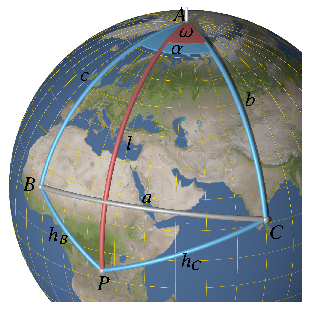
\includegraphics{papers/nav/images/position/position1-small.pdf}}%
}
\medskip

\subsection{Koordinaten der Bildpunkte}
Als erstes benötigen wir die Koordinaten der Bildpunkte von Arktur und Deneb. 
$\delta$ ist die Breite, $\lambda$ die Länge.
\begin{align}
\delta_{\text{Deneb}}&=DEC_{\text{Deneb}} = \underline{\underline{45.361194^\circ}} \nonumber \\ 
\lambda_{\text{Deneb}}&=RA_{\text{Deneb}} - s = 310.55058^\circ -118.610804^\circ =\underline{\underline{191.939776^\circ}}   \nonumber \\ 
\delta_{\text{Arktur}}&=DEC_{\text{Arktur}} =  \underline{\underline{19.063222^\circ}} \nonumber \\ 
\lambda_{\text{Arktur}}&=RA_{\text{Arktur}} - s = 214.17558^\circ -118.610804^\circ = \underline{\underline{5.5647759^\circ}}  \nonumber  
\end{align}


\subsection{Dreiecke definieren}
\begin{figure} 
\hbox{%
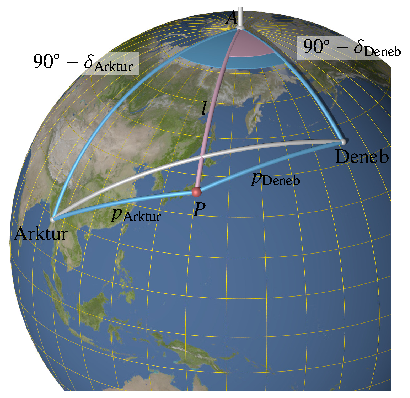
\includegraphics{papers/nav/images/beispiele/beispiele1.pdf}%
\hfill%
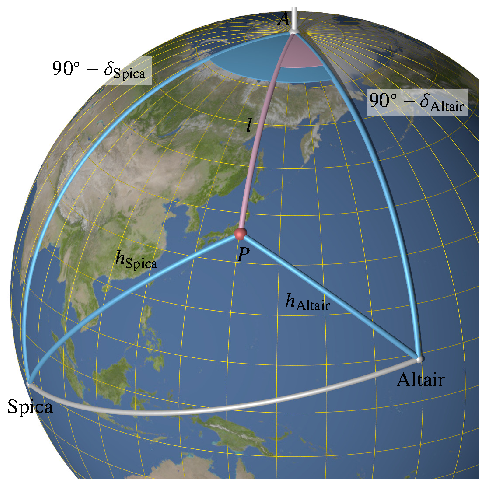
\includegraphics{papers/nav/images/beispiele/beispiele2.pdf}}
\caption{Arktur-Deneb; Spica-Altiar
\label{nav:beispiele}}
\end{figure}
Das Festlegen der Dreiecke ist essenziell für die korrekten Berechnungen.
Ein Problem, welches in der Theorie nicht berücksichtigt wurde ist, dass der Punkt $P$ nicht zwingend unterhalb der Seite $a$ sein muss. 
Wenn man das nicht berücksichtigt, erhält man falsche oder keine Ergebnisse. 
In der Realität weiss man jedoch ungefähr auf welchem Breitengrad man ist, so kann man relativ einfach entscheiden, ob der eigene Standort über $a$ ist oder nicht.
Beim unserem genutzten Paar Arktur-Deneb ist dies kein Problem, da der Punkt unterhalb der Seite $a$ liegt. 
Würde man aber das Paar Altair-Spica nehmen, liegt $P$ über $a$
(vgl. Abbildung\ref{nav:beispiele}) und man müsste trigonometrisch
anders vorgehen. 

\subsection{Dreieck $ABC$}
\vspace*{-3mm}
\hbox to\textwidth{%
\begin{minipage}{8.4cm}%
Nun berechnen wir alle Seitenlängen $a$, $b$, $c$ und die
Innnenwinkel $\alpha$, $\beta$ und $\gamma$.
Wir können $b$ und $c$ mit den geltenten Zusammenhängen des nautischen Dreiecks wie folgt bestimmen:
\begin{align*}
b
&=
90^\circ-DEC_{\text{Deneb}}
=
90^\circ - 45.361194^\circ
\\
&=
\underline{\underline{44.638806^\circ}}
\\
c
&=
90^\circ-DEC_{\text{Arktur}}
=
90^\circ - 19.063222^\circ
\\
&=
\underline{\underline{70.936778^\circ}}
\end{align*}
\end{minipage}%
\hfill%
\raisebox{-2.4cm}{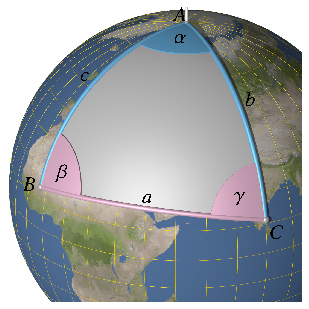
\includegraphics{papers/nav/images/position/position2-small.pdf}}%
}
Um $a$ zu bestimmen, benötigen wir zuerst den Winkel
\begin{align*}
\alpha
&=
RA_{\text{Deneb}} - RA_{\text{Arktur}}
=
310.55058^\circ -214.17558^\circ
\\
&=
\underline{\underline{96.375^\circ}}.
\end{align*}
Danach nutzen wir den sphärischen Winkelkosinussatz, um  $a$ zu berechnen:
\begin{align*}
	a &= \cos^{-1}(\cos(b) \cdot \cos(c) + \sin(b) \cdot \sin(c) \cdot \cos(\alpha)) \\
	 &= \cos^{-1}(\cos(44.638806^\circ) \cdot \cos(70.936778^\circ) + \sin(44.638806^\circ) \cdot \sin(70.936778^\circ) \cdot \cos(96.375^\circ)) \\
	 &= \underline{\underline{80.8707801^\circ}}
\end{align*}
Für $\beta$ und $\gamma$ nutzen wir den sphärischen Seitenkosinussatz:
\begin{align*}
	\beta &= \cos^{-1}  \bigg[\frac{\cos(b)-\cos(a) \cdot \cos(c)}{\sin(a) \cdot \sin(c)}\bigg] \\
	&= \cos^{-1}  \bigg[\frac{\cos(44.638806^\circ)-\cos(80.8707801^\circ) \cdot \cos(70.936778^\circ)}{\sin(80.8707801^\circ) \cdot \sin(70.936778^\circ)}\bigg] \\
	&= \underline{\underline{45.0115314^\circ}} 
\\
\gamma &=  \cos^{-1}  \bigg[\frac{\cos(c)-\cos(b) \cdot \cos(a)}{\sin(a) \cdot \sin(b)}\bigg] \\
	&=  \cos^{-1}  \bigg[\frac{\cos(70.936778^\circ)-\cos(44.638806^\circ) \cdot \cos(80.8707801^\circ)}{\sin(80.8707801^\circ) \cdot \sin(44.638806^\circ)}\bigg] \\
	&=\underline{\underline{72.0573328^\circ}} 
\end{align*}



\subsection{Dreieck $BPC$}
\vspace*{-4mm}
\hbox to\textwidth{%
\begin{minipage}{8.4cm}%
Als nächstes berechnen wir die Seiten $p_B$, $p_B$ und die Innenwinkel $\beta_1$ und $\gamma_1$.
\begin{align*}
p_B&=90^\circ - h_B 
	= 90^\circ - 47.42744^\circ \\
	&= \underline{\underline{42.572556^\circ}} 
\\
	p_C &= 90^\circ - h_C 
	= 90^\circ - 50.256027^\circ \\
	&= \underline{\underline{39.743973^\circ}} 
\end{align*}
\end{minipage}%
\hfill%
\raisebox{-2.8cm}{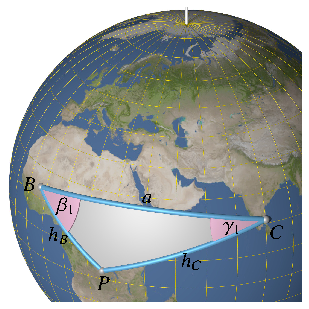
\includegraphics{papers/nav/images/position/position3-small.pdf}}%
}
\begin{align*}
\beta_1 &= \cos^{-1}  \bigg[\frac{\cos(p_c)-\cos(a) \cdot \cos(p_B)}{\sin(a) \cdot \sin(p_B)}\bigg] \\
	&= \cos^{-1}  \bigg[\frac{\cos(39.743973^\circ)-\cos(80.8707801^\circ) \cdot \cos(42.572556^\circ)}{\sin(80.8707801^\circ) \cdot \sin(42.572556^\circ)}\bigg] \\
	&=\underline{\underline{12.5211127^\circ}} 
\\
\gamma_1 &= \cos^{-1}  \bigg[\frac{\cos(p_b)-\cos(a) \cdot \cos(p_C)}{\sin(a) \cdot \sin(p_C)}\bigg] \\
	&= \cos^{-1}  \bigg[\frac{\cos(42.572556^\circ)-\cos(80.8707801^\circ) \cdot \cos(39.743973^\circ)}{\sin(80.8707801^\circ) \cdot \sin(39.743973^\circ)}\bigg] \\
	&=\underline{\underline{13.2618475^\circ}} 
\end{align*}

\subsection{Dreieck $ABP$}
\vspace*{-2mm}
\hbox to\textwidth{%
\begin{minipage}{8.4cm}%
Als erstes müssen wir den Winkel $\beta_2$ berechnen:
\begin{align*}
	\beta_2 &= \beta + \beta_1 = 45.011513^\circ + 12.5211127^\circ \\
	&=\underline{\underline{44.6687451^\circ}} 
\end{align*}
Danach können wir mithilfe von $\beta_2$, $c$ und $p_B$ die Seite $l$ berechnen:
\begin{align*}
l
&=
\cos^{-1}(\cos(c) \cdot \cos(p_B)
          + \sin(c) \cdot \sin(p_B) \cdot \cos(\beta_2)) \\
&=
\cos^{-1}(\cos(70.936778^\circ) \cdot \cos(42.572556^\circ)\\
&\qquad + \sin(70.936778^\circ) \cdot \sin(42.572556^\circ) \cdot \cos(57.5326442^\circ)) \\
&= \underline{\underline{54.2833404^\circ}} 
\end{align*}
\end{minipage}%
\hfill%
\raisebox{-2.0cm}{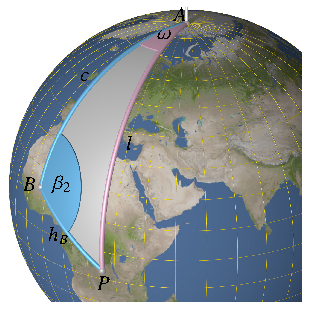
\includegraphics{papers/nav/images/position/position4-small.pdf}}%
}

\medskip

Damit wir gleich den Längengrad berechnen können, benötigen wir noch den Winkel $\omega$:
\begin{align*}
	\omega &= \cos^{-1}  \bigg[\frac{\cos(p_B)-\cos(c) \cdot \cos(l)}{\sin(c) \cdot \sin(l)}\bigg] \\
	&=\cos^{-1}  \bigg[\frac{\cos(42.572556^\circ)-\cos(70.936778^\circ) \cdot \cos(54.2833404^\circ)}{\sin(70.936778^\circ) \cdot \sin(54.2833404^\circ)}\bigg] \\
	&= \underline{\underline{44.6687451^\circ}} 
\end{align*}

\subsection{Längengrad und Breitengrad bestimmen}

\begin{align*}
\delta &= 90^\circ - l &
	\lambda &= \lambda_{\text{Arktur}} + \omega \\
&= 90^\circ - 54.2833404 &
	&= 95.5647759^\circ + 44.6687451^\circ \\
&= \underline{\underline{35.7166596^\circ}} &
	&= \underline{\underline{140.233521^\circ}} 
\end{align*}
Wie wir sehen, stimmen die berechneten Koordinaten mit den Koordinaten des Punktes, an welchem gemessen wurde überein. 

\subsection{Fazit}
Die theoretische Anleitung im Abschnitt \ref{sta} scheint grundsätzlich zu funktionieren. 
Allerdings gab es zwei interessante Probleme.

Einerseits das Problem, ob der Punkt $P$ sich oberhalb oder unterhalb von $a$ befindet. 
Da wir eigentlich wussten, wo der gesuchte Punkt $P$ ist, konnten wir das Dreieck anhand der Koordinaten der Bildpunkte richtig aufstellen. 
In der Praxis muss man aber schon wissen, auf welchem Breitengrad man ungefähr ist. 
Dies weis man in der Regeln aber, da die eigene Breite die Höhe des Polarsterns ist.
Diese Höhe wird mit dem Sextant gemessen.

Andererseits ist da noch ein Problem mit dem Sinussatz.
Beim Sinussatz gibt es immer zwei Lösungen, weil \[ \sin(\pi-a)=\sin(a).\]
Da kann es sein (und war in unserem Fall auch so), dass man das falsche Ergebnis erwischt. 
Wegen dieser Erkenntnis haben wir nur Kosinussätze verwendet und dies ebenfalls im Abschnitt \ref{sta} abgeändert, da es für den Leser auch relevant sein kann, wenn er es Probieren möchte.




